% For LaTeX-Box: root = stat105_F15_exam1B.tex 
%%%%%%%%%%%%%%%%%%%%%%%%%%%%%%%%%%%%%%%%%%%%%%%%%%%%%%%%%%%%%%%%%%%%%%%%%%%%%%%%
%  File Name: stat105_F15_exam1B.tex
%  Purpose:
%
%  Creation Date: 24-09-2015
%  Last Modified: Tue Sep 29 10:42:14 2015
%  Created By:
%%%%%%%%%%%%%%%%%%%%%%%%%%%%%%%%%%%%%%%%%%%%%%%%%%%%%%%%%%%%%%%%%%%%%%%%%%%%%%%%
\documentclass[addpoints]{examsetup}\usepackage[]{graphicx}\usepackage[]{color}
%% maxwidth is the original width if it is less than linewidth
%% otherwise use linewidth (to make sure the graphics do not exceed the margin)
\makeatletter
\def\maxwidth{ %
  \ifdim\Gin@nat@width>\linewidth
    \linewidth
  \else
    \Gin@nat@width
  \fi
}
\makeatother

\definecolor{fgcolor}{rgb}{0.345, 0.345, 0.345}
\newcommand{\hlnum}[1]{\textcolor[rgb]{0.686,0.059,0.569}{#1}}%
\newcommand{\hlstr}[1]{\textcolor[rgb]{0.192,0.494,0.8}{#1}}%
\newcommand{\hlcom}[1]{\textcolor[rgb]{0.678,0.584,0.686}{\textit{#1}}}%
\newcommand{\hlopt}[1]{\textcolor[rgb]{0,0,0}{#1}}%
\newcommand{\hlstd}[1]{\textcolor[rgb]{0.345,0.345,0.345}{#1}}%
\newcommand{\hlkwa}[1]{\textcolor[rgb]{0.161,0.373,0.58}{\textbf{#1}}}%
\newcommand{\hlkwb}[1]{\textcolor[rgb]{0.69,0.353,0.396}{#1}}%
\newcommand{\hlkwc}[1]{\textcolor[rgb]{0.333,0.667,0.333}{#1}}%
\newcommand{\hlkwd}[1]{\textcolor[rgb]{0.737,0.353,0.396}{\textbf{#1}}}%

\usepackage{framed}
\makeatletter
\newenvironment{kframe}{%
 \def\at@end@of@kframe{}%
 \ifinner\ifhmode%
  \def\at@end@of@kframe{\end{minipage}}%
  \begin{minipage}{\columnwidth}%
 \fi\fi%
 \def\FrameCommand##1{\hskip\@totalleftmargin \hskip-\fboxsep
 \colorbox{shadecolor}{##1}\hskip-\fboxsep
     % There is no \\@totalrightmargin, so:
     \hskip-\linewidth \hskip-\@totalleftmargin \hskip\columnwidth}%
 \MakeFramed {\advance\hsize-\width
   \@totalleftmargin\z@ \linewidth\hsize
   \@setminipage}}%
 {\par\unskip\endMakeFramed%
 \at@end@of@kframe}
\makeatother

\definecolor{shadecolor}{rgb}{.97, .97, .97}
\definecolor{messagecolor}{rgb}{0, 0, 0}
\definecolor{warningcolor}{rgb}{1, 0, 1}
\definecolor{errorcolor}{rgb}{1, 0, 0}
\newenvironment{knitrout}{}{} % an empty environment to be redefined in TeX

\usepackage{alltt}

\usepackage{etoolbox}
\usepackage{tikz,pgfplots}

%% For LaTeX-Box: root = stat105_exam1_info.tex 
%%%%%%%%%%%%%%%%%%%%%%%%%%%%%%%%%%%%%%%%%%%%%%%%%%%%%%%%%%%%%%%%%%%%%%%%%%%%%%%%
%  File Name: stat105_exam1_info.tex
%  Purpose:
%
%  Creation Date: 24-09-2015
%  Last Modified: Thu Sep 24 13:51:36 2015
%  Created By:
%%%%%%%%%%%%%%%%%%%%%%%%%%%%%%%%%%%%%%%%%%%%%%%%%%%%%%%%%%%%%%%%%%%%%%%%%%%%%%%%
\newcommand{\course}[1]{\ifstrempty{#1}{STAT 105}{STAT 105, Section #1}}
\newcommand{\sectionNumber}{B}
\newcommand{\examDate}{October 1, 2015}
\newcommand{\semester}{FALL 2015}
\newcommand{\examNumber}{II}

\newcommand{\examTitle}{Exam \examNumber}

\runningheader{\course{\sectionNumber}}{Exam \examNumber}{\examDate}
\runningfooter{}{}{Page \thepage of \numpages}

\newcommand{\examCoverPage}{
   \begin{coverpages}
   \centering
   {\bfseries\scshape\Huge Exam I \par}
   \vspace{1cm}
   {\bfseries\scshape\LARGE \course{\sectionNumber} \par}
   {\bfseries\scshape\LARGE \semester \par}

   \vspace{2cm}

   \fbox{\fbox{\parbox{5.5in}{\centering 

      \vspace{.25cm} 
      
      {\bfseries\Large Instructions} \\

      \vspace{.5cm} 

      \begin{itemize}
         \item  The exam is scheduled for 80 minutes, from 8:00 to 9:20 AM. At 9:20 AM the exam will end.\\
         \item  A forumula sheet is attached to the end of the exam. Feel free to tear it off.\\
         \item  You may use a calculator during this exam.\\
         \item  Answer the questions in the space provided. If you run out of room, continue on the back of the page. \\
         \item  If you have any questions about, or need clarification on the meaning of an item on this exam, please ask your instructor. No other form of external help is permitted attempting to receive help or provide help to others will be considered cheating.\\
         \item  {\bfseries Do not cheat on this exam.} Academic integrity demands an honest and fair testing environment. Cheating will not be tolerated and will result in an immediate score of 0 on the exam and an incident report will be submitted to the dean's office.\\
      \end{itemize}

   }}}

   \vspace{2cm}

   \makebox[0.6\textwidth]{Name:\enspace\hrulefill}

   \vspace{1cm}

   \makebox[0.6\textwidth]{Student ID:\enspace\hrulefill}
   \end{coverpages}

}


\newcommand{\course}[1]{\ifstrempty{#1}{STAT 105}{STAT 105, Section #1}}
\newcommand{\sectionNumber}{B}
\newcommand{\examDate}{October 1, 2015}
\newcommand{\semester}{FALL 2015}
\newcommand{\examNumber}{I}

%%%%%%%%%%%%%%%%%%%%%%%%%%%%%%%%%%%%%%%%%%%%%%%%%%%%%%%%%%%%%%%%%%%%%%%%%%%%%%%%
\IfFileExists{upquote.sty}{\usepackage{upquote}}{}
\begin{document}

%-- : R code (Code in Document)



\examCoverPage

\begin{questions}

\question[2] 

Circle the \textbf{bold face} term that makes the following statement true: \\

A measurement device that reports the true measurement of the item on which the device is being used is (\textbf{precise} or \textbf{accurate}).

\vspace{1cm}

\question 

%-- : R code (Code in Document)


A sample of size 5 was drawn from a population and the resulting observations are reported below. 
\begin{center}
12, 15, 18, 19, 26
\end{center}
Using these observed values, report the following:
\vspace{1cm}

\begin{parts}

   \part[2] the mean  
   \vspace{2cm}

   \part[2] the median 
   \vspace{2cm}

   \part[2] the variance 
   \vspace{2cm}

   \part[2] the standard deviation 
   \vspace{2cm}

   \part[2] the value of $Q(.25)$
   \vspace{2cm}

   \part[2] the Interquartile Range
   \vspace{2cm}

\end{parts}

\question

An environmental engineer is testing four methods for reducing the concentration of a certain lake pollutant found in Iowa lakes.
To do this he first randomly selected 20 Iowa lakes from which he took water samples,
then split each of the 20 samples into 4 portions, 
and randomly labeled the four portions 1, 2, 3, and 4. 
Finally, he attempted to reduce the concentration of each 
of the portions labeled 1 using the the first method, 
of each of the portions labeled 2 using the second method, 
of each of the portions labeled 3 using the third method, 
and of each of the portions labeled portion 4 using the fourth method. 
After the methods had been applied, he measured the change in concentration. \\

\begin{parts}
   \part[2] Is this an experiment or an observational study? Explain.

  \vspace{2cm}

   \part Identify the following (if there was not one, simply put "not used").

  \vspace{1cm}

   \begin{subparts}
      \subpart[2] Response variable(s):

      \vspace{2cm}

      \subpart[2] Experimental variable(s):

      \vspace{2cm}

      \subpart[2] Blocking variable(s):

      \vspace{2cm}

   \end{subparts}

   \part[2] Was replication used in this experiment? If so, where was it applied? If not, how could we have applied it?

  \vspace{2cm}

\end{parts}

\pagebreak

\question

Recently my teenage niece had an opportunity to upgrade her smart phone. 
She narrowed her choices down to two phones (phone A and phone B) but had a hard time making her final decision.
She decided to ask people she knew who had one of the phones to rate their satisfaction from 0\% to 100\%.
She also asked them if they would prefer to have the other phone.
In order to help put their feelings in perspective, she also made note of how negative she thought they were in general, 
using three descriptions: the interviewee was classified as overly critical, appropriately critical, or not critical enough. 

\begin{parts}
   \part[2] Is this an experiment or an observational study?

   \vspace{2cm}
   \part[2] Identify the response variable(s).

   \vspace{2cm}
   \part For each of the following variables, 

   \begin{itemize}

      \item Identify whether it is qualitative or quantitative variable, and 

      \item If it is qualitative, what are the possible values it can take? If it is quantitative, is it continuous or discrete?

   \end{itemize}

   \begin{subparts}

      \subpart the individual's reported phone satisfaction percentage.

      \vspace{2cm}

      \subpart my niece's appraisal of the interviewee's negativity.

      \vspace{2cm}

      \subpart whether or not the interviewee would prefer to have the other phone.

      \vspace{2cm}

      \subpart the type of phone the interviewee currently owns.

   \end{subparts}

\end{parts}
\pagebreak

\question 

%-- : R code (Code in Document)


The strength of an internet connection is often described in terms of its download speed, measured in megabits per second (or Mbps).
A systems administrator is concerned that recent changes in her company's main server framework may be having a negative impact on the local network's download speed.
Every 2 minutes for an hour, she recorded the network speed at that moment and collected her results into the following stem-and-leaf plot:

%-- : R code (Code in Document)
\begin{knitrout}
\definecolor{shadecolor}{rgb}{0.969, 0.969, 0.969}\color{fgcolor}\begin{kframe}
\begin{verbatim}

  The decimal point is at the |

   0 | 9
   1 | 8
   2 | 7
   3 | 6
   4 | 134
   5 | 7
   6 | 1145677
   7 | 01338
   8 | 2346
   9 | 79
  10 | 45
  11 | 
  12 | 17
\end{verbatim}
\end{kframe}
\end{knitrout}

Note that \verb!0 | 9! represents 0.9. In this case, the first quartile is $Q(.25) = 5.7$, the median is 6.85, and the IQR is 2.7.

\begin{parts}
  \part[10] Complete the following frequency table: \\

  \begin{table}[h!]
     \centering
     \begin{tabular}{|l|p{3cm}|p{3cm}|p{4cm}|}
        \hline
                             & \textbf{Frequency} & \textbf{Relative} & \textbf{Cumulative}  \\
        \textbf{Value Range} &                    & \textbf{Frequency} & \textbf{Relative Frequency} \\\hline \hline
                    &  &  &  \\
      0.00 - 2.00   &  &  &  \\
                    &  &  &  \\ \hline
                    &  &  &  \\
      2.01 - 4.00   &  &  &  \\
                    &  &  &  \\ \hline
                    &  &  &  \\
      4.01 - 6.00   &  &  &  \\
                    &  &  &  \\ \hline
                    &  &  &  \\
      6.01 - 8.00   &  &  &  \\
                    &  &  &  \\ \hline
                    &  &  &  \\
      8.01 - 10.00  &  &  &  \\
                    &  &  &  \\ \hline
                    &  &  &  \\
      10.01 - 12.00 &  &  &  \\
                    &  &  &  \\ \hline
                    &  &  &  \\
      12.01 - 14.00 &  &  &  \\
                    &  &  &  \\  \hline
     \end{tabular}
  \end{table}

  \pagebreak

  \part[10] Create a box plot to summarize the data. Carefully label the axes.

  \vspace{7cm}

  \part[4] Are there any unusually low observations? If so What were the speeds at those points?

  \vspace{3cm}

  \part[10] She also measured upload speed, obtaining the following 8 values.

%-- : R code (Code in Document)


\begin{center}
   7.45, 4.22, 7.7, 6.04, 7.68, 5.71, 4.71, 8.44
\end{center}

Create a theoretical Q-Q plot using the following quantiles from the normal distribution as the theoretical quantiles. Carefully label your axes.
What does this graph tell us about the upload speeds?

\begin{table}[h!]
   \centering
   \begin{tabular}{ccccccccc}
             & 1 & 2 & 3 & 4 & 5 & 6 & 7 & 8 \\ \hline
      $p$    & 0.0625 & 0.1875 & 0.3125 & 0.4375 & 0.5625 & 0.6875 & 0.8125 & 0.9375 \\
      $Q(p)$ & \ensuremath{-1.53} & \ensuremath{-0.89} & \ensuremath{-0.49} & \ensuremath{-0.16} & 0.16 & 0.49 & 0.89 & 1.53 \\ \hline
   \end{tabular}
\end{table}


\end{parts}
\pagebreak

\question

The major cause of axel failure in freight trucks is when shippers exceed the recommended weight limits that can be handled by the axels. 
Issues resulting from these failures have been becoming more frequent as shippers try to cut corners, 
leading members of the state's Department of Transportation to ask one of their civil engineers 
to look into the available data and better advise them on the relationship between excessive weight and axel failure.

A company manufacturing axels provides the engineer with data gathered from conducting experiments loading axels with excessive weight and simulating traveling conditions.
The data consists of two columns, \textbf{excessive weight (in tonnes)} is the amount of weight over the limit that was placed on the axel, and 
\textbf{distance to failure (in tens of thousands of miles)} is the simulated distance to the axel's failure. 

%-- : R code (Code in Document)


\begin{center}
\begin{knitrout}
\definecolor{shadecolor}{rgb}{0.969, 0.969, 0.969}\color{fgcolor}
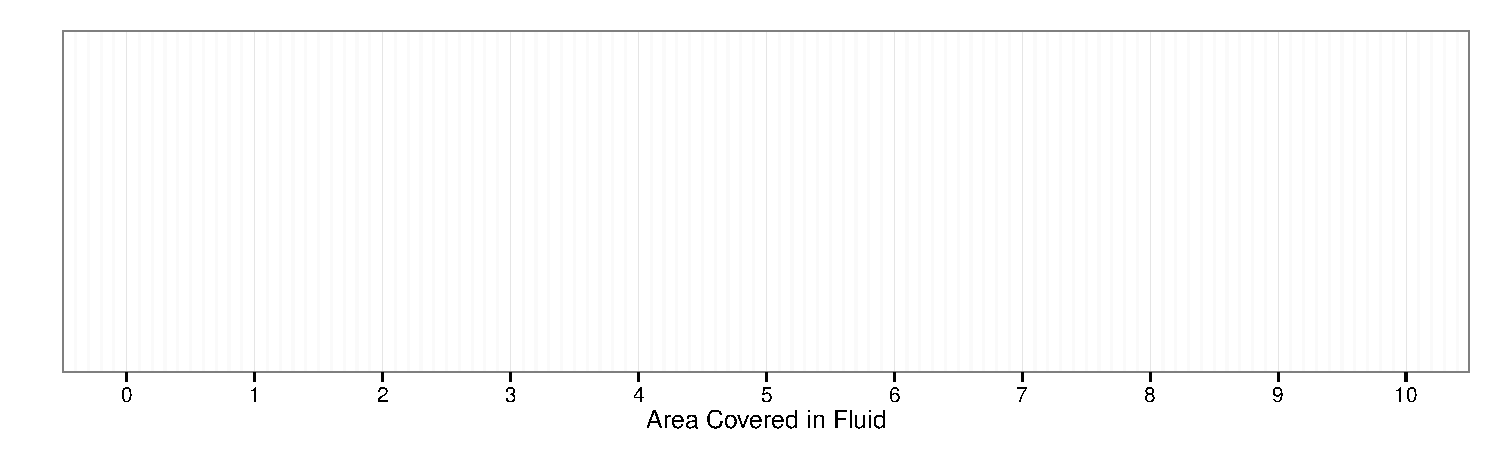
\includegraphics[width=.5\linewidth]{figure/unnamed-chunk-7-1} 

\end{knitrout}
\end{center}

Here are some summaries of the data:

$$
\sum_{i=1}^{50} x_i = 64 \hspace{3cm} \sum_{i=1}^{50} x_i^2 = 107 \\
$$

$$
\sum_{i=1}^{50} y_i = 2008 \hspace{3cm} \sum_{i=1}^{50} y_i^2 = 95182 \\
$$

$$
\sum_{i=1}^{50} x_i y_i = 1999
$$

\begin{parts}
   \part Using the summaries above, fit a linear relationship between \textbf{weight exceeding guidelines} (x) and \textbf{travel distance to failure} (y). 
   \begin{subparts}
      \subpart[5] Write the equation of the fitted linear relationship. 
      \vspace{2cm}
      \subpart[5] Find and interpret the value of $R^2$ for the fitted linear relationship.
      \vspace{2cm}
      \subpart[5] Using the fitted line, provide a predicted value of travel distance to failure when the weight exceeding the guidelines is 3.4 tonnes.
      \vspace{2cm}
   \end{subparts}

   \part The JMP output below comes from fitting a quadratic model using $x$ and $x^2$. 

   \centerline{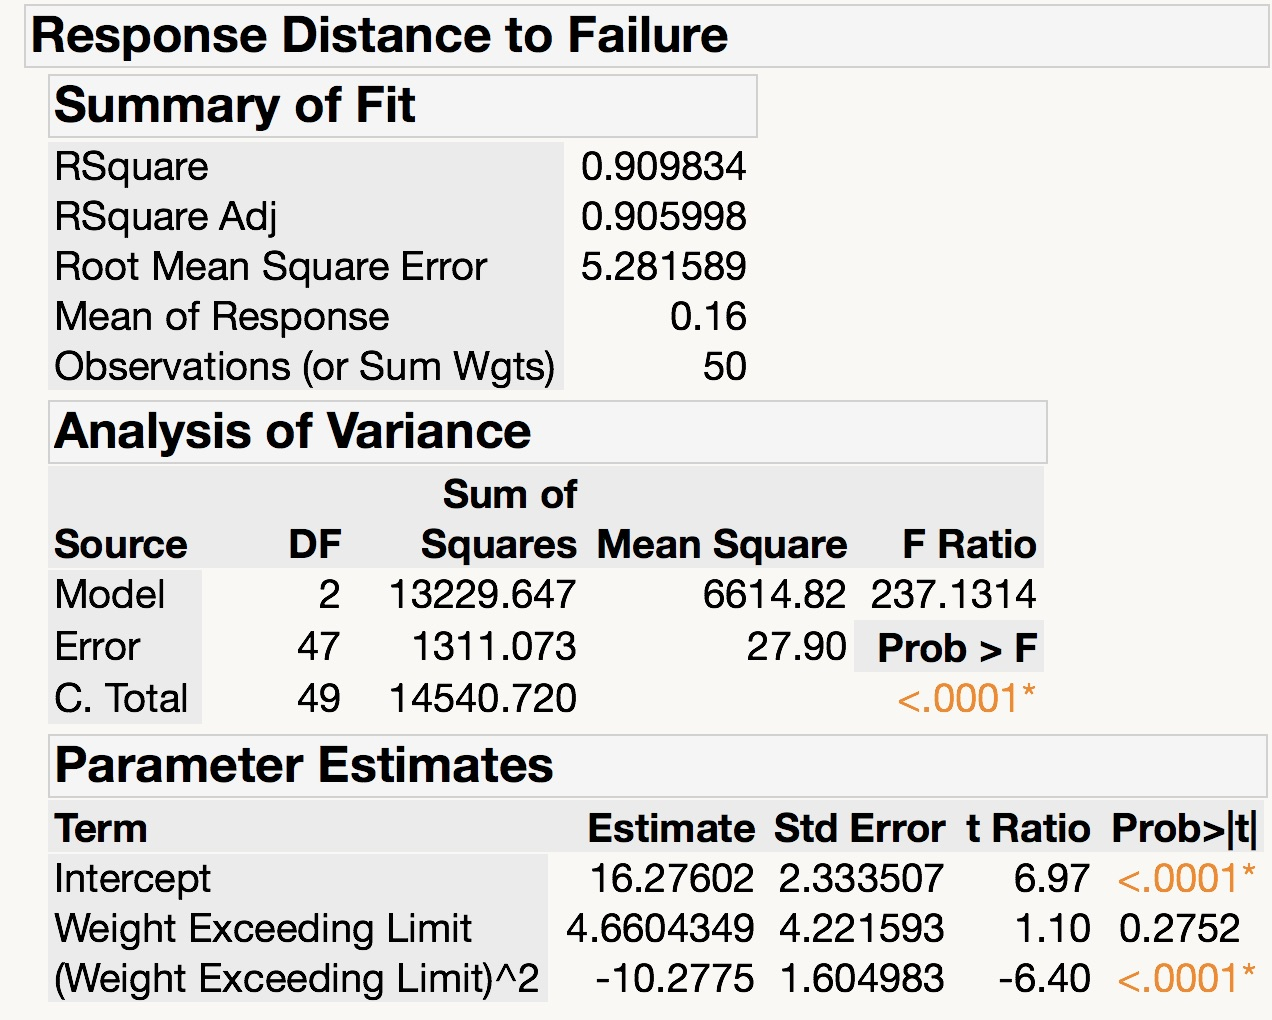
\includegraphics[scale=.2]{FitModel}}

   \begin{subparts}
      \subpart[5] Write the equation of the fitted quadratic relationship. 
      \vspace{2cm}
      \subpart[5] Find and interpret the value of $R^2$ for the fitted quadratic relationship.
      \vspace{2cm}
      \subpart[5] Using the fitted quadratic relationship, provide a predicted value of travel distance to failure when the weight exceeding the guidelines is 3.4 tonnes.
   \end{subparts}
\end{parts}

\end{questions}

\end{document}
